%Solución del Ejercicio 4 por medio de la metodología 6D

\subsection{Descripción del problema}
Dado un numero decimal entero positivo o negativo regresar su equivalente en binario.

\begin {figure}[h!]
\centerline{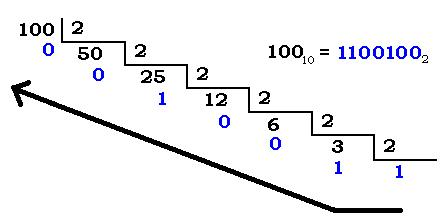
\includegraphics[width = 6cm]{Latex-imágenes/Conversion.jpeg}}
\caption{Conversión a Binario.}
\label{fig}
\end {figure}

\subsection{Definición de la solución}
Para obtener un número binario, se requiere realizar una serie de operaciones. Consiste en la división sucesiva del número decimal por dos, obteniendo el residuo en cada paso. Luego, los residuos se combinan en orden inverso para formar el número binario correspondiente. Este proceso se repite hasta que el cociente de la división sea igual a cero. Sin embargo, esta metodología presenta una problemática debido a su ineficiencia y el riesgo de cometer errores en los cálculos.

La solución planteada para abordar esta problemática ha sido la creación de una técnica computacional en el lenguaje de programación Java. Este diseño automatiza y asegura la conversión de números enteros positivos y negativos a su equivalente en el sistema binario de manera precisa y confiable. 

\subsection{Diseño de la solución}
\begin {figure}[htb]
\centerline{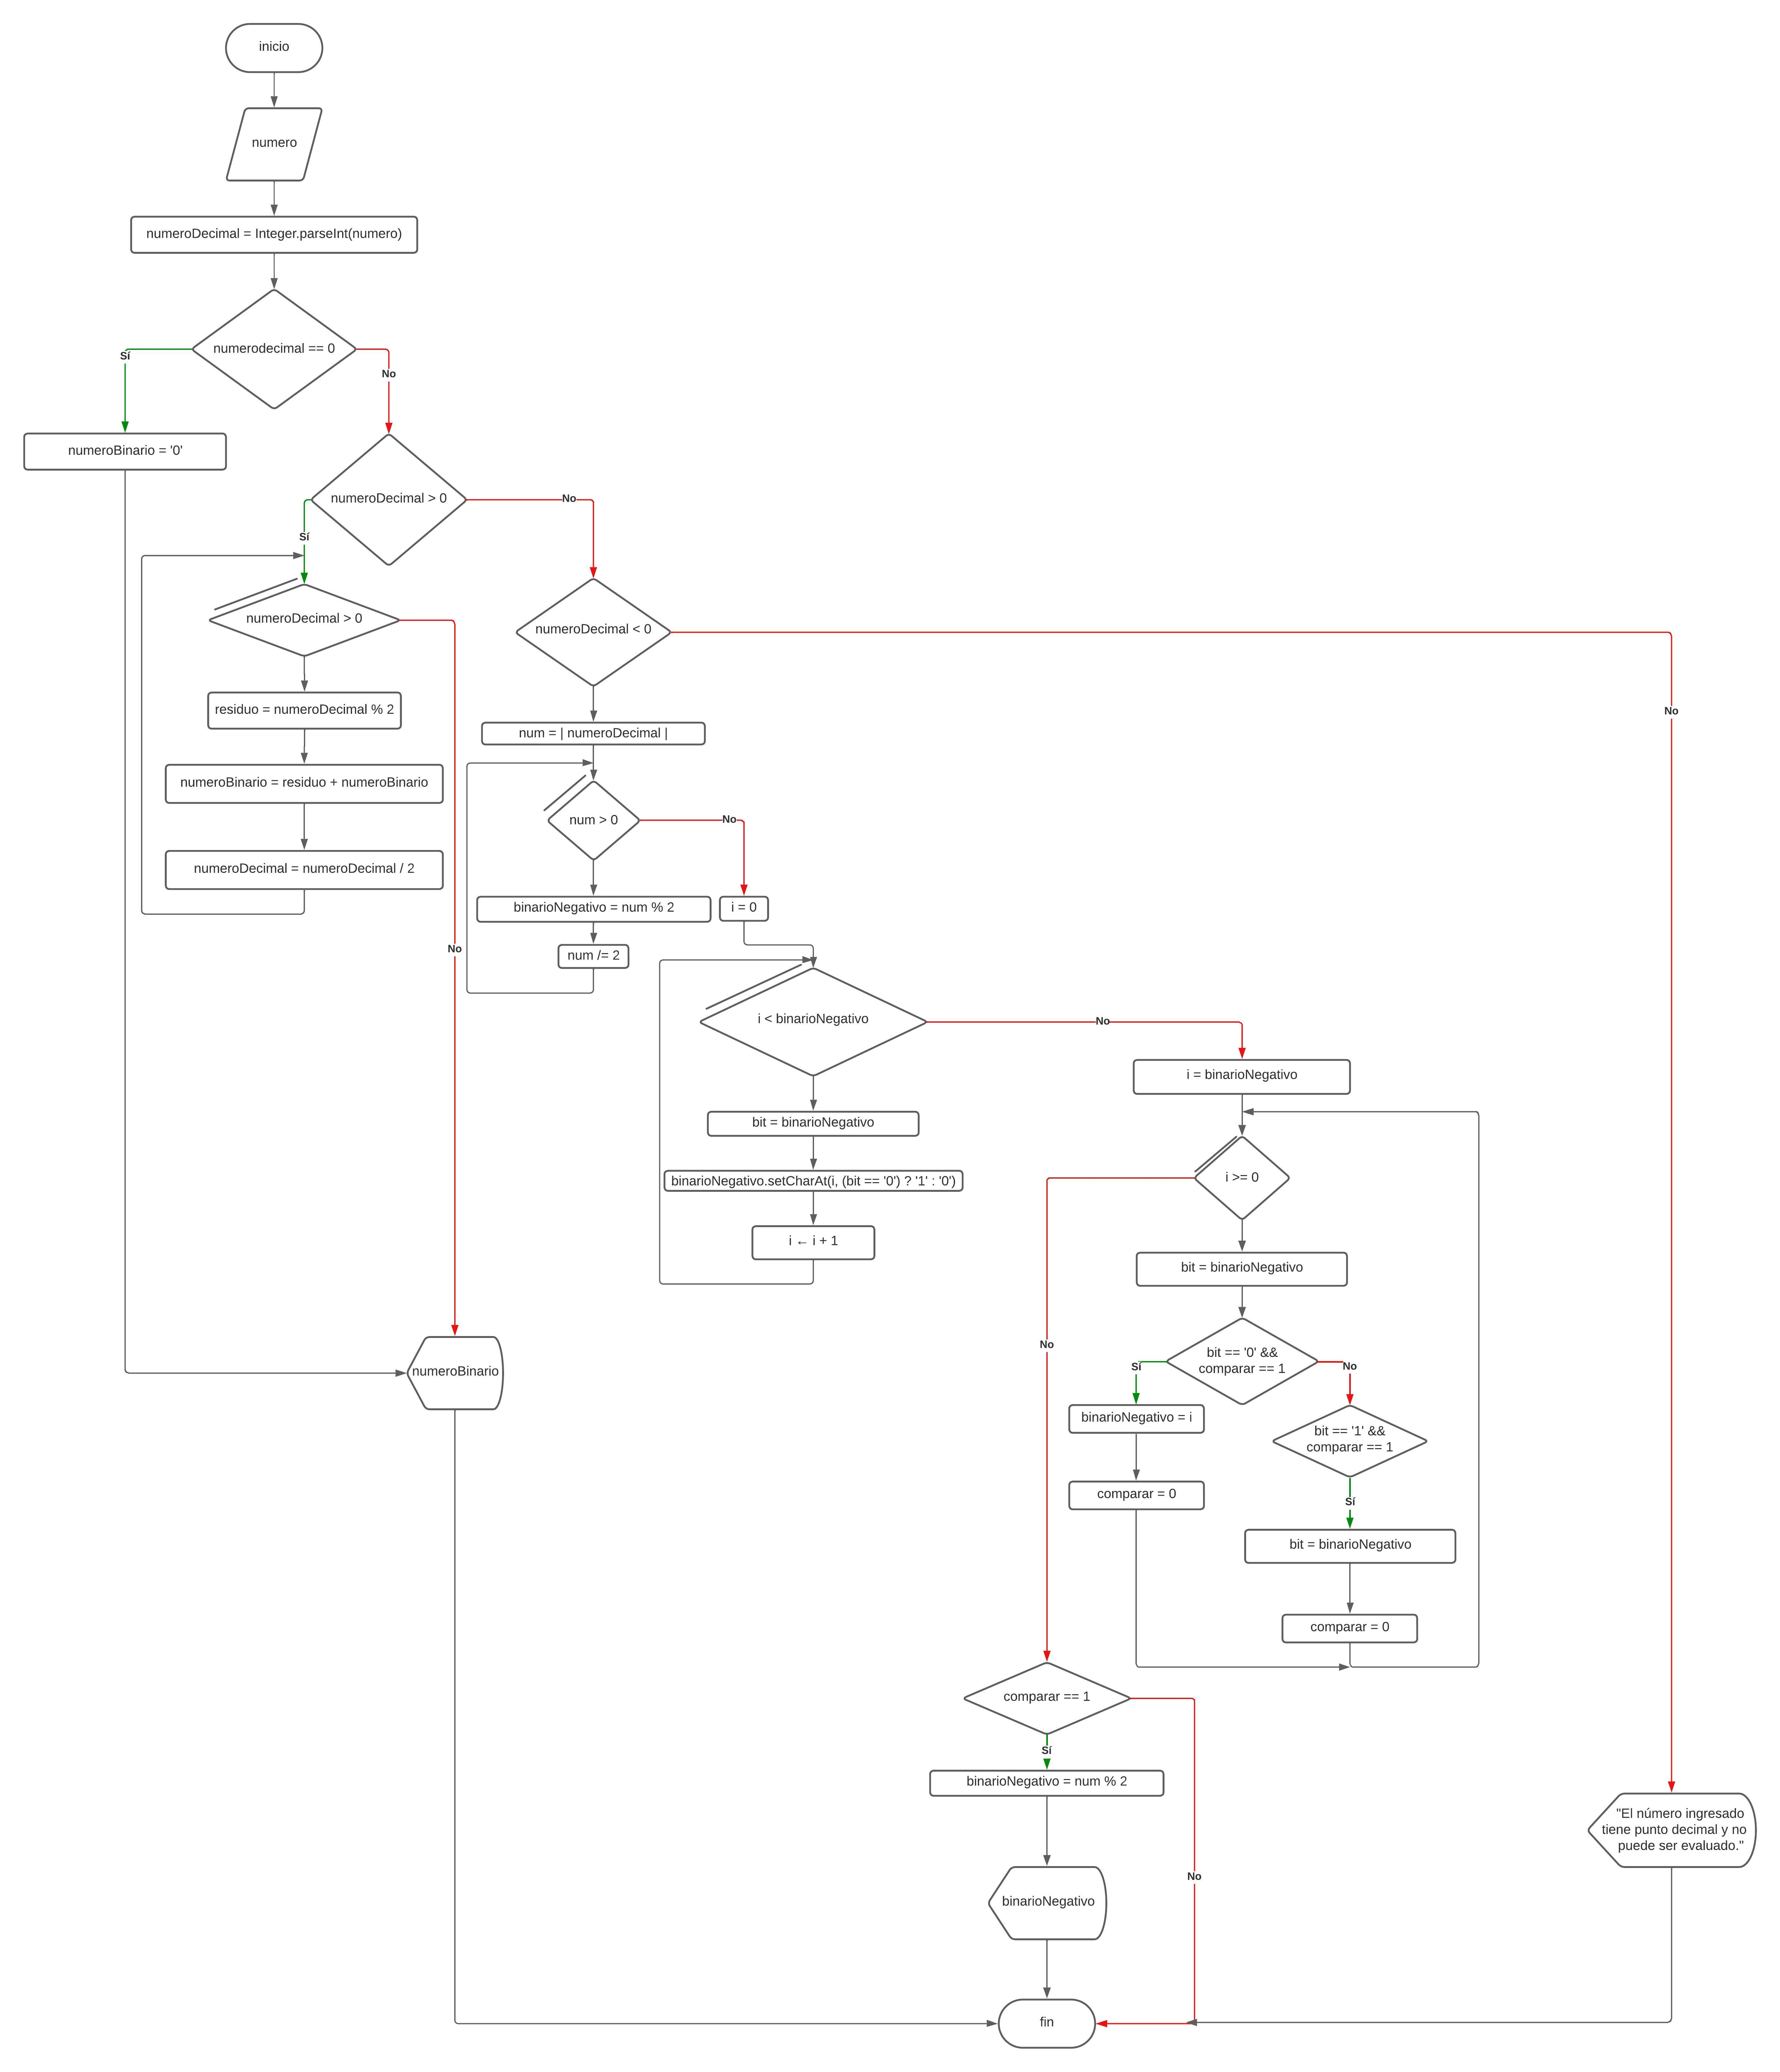
\includegraphics[width = 6cm]{Latex-imágenes/diagramaEx4.jpeg}}
\caption{Representación gráfica del algoritmo implementando la solución}
\label{fig}
\end {figure}


\subsection{Desarrollo de la solución}
En este bloque de código, se solicita al usuario que ingrese un número entero, ya sea positivo o negativo, para luego utilizarlo.
\begin{javaCode}
import javax.swing.JOptionPane;

public class decimalBinario {

    public static void main(String[] args) {
        String numero = JOptionPane.showInputDialog("Ingrese un número decimal:");
        try {
            int numeroDecimal = Integer.parseInt(numero);
            String numeroBinario = "";
\end{javaCode}
En el siguiente bloque de código se realiza una comparación con el número ingresado anteriormente. Dentro de las estructuras condicionales, se encuentra un ciclo que se encarga de descomponer el número entero en su respectiva representación binaria.
\begin{javaCode}
    if (numeroDecimal == 0) {
                numeroBinario = "0";
            } else if(numeroDecimal > 0){
                while (numeroDecimal > 0) {
                    int residuo = numeroDecimal % 2;
                    numeroBinario = residuo + numeroBinario;
                    numeroDecimal = numeroDecimal / 2;
                }
            }else 
\end{javaCode}
En este bloque de código se presenta una condición en la que, si el número entero ingresado es negativo, se realizará la conversión a su representación binaria utilizando el método del complemento A2. El complemento A2 es una operación utilizada para representar números negativos en sistemas binarios.
\begin{javaCode}
if(numeroDecimal < 0){
StringBuilder binarioNegativo = new StringBuilder();
int num = Math.abs(numeroDecimal);

while (num > 0) {
binarioNegativo.insert(0, num % 2);
num /= 2;
}
for (int i = 0; i < binarioNegativo.length(); i++) {
char bit = binarioNegativo.charAt(i);
binarioNegativo.setCharAt(i, (bit == '0') ? '1' : '0');
}

int comparar = 1;
for (int i = binarioNegativo.length() - 1; i >= 0; i--) {
char bit = binarioNegativo.charAt(i);
if (bit == '0' && comparar == 1) {
binarioNegativo.setCharAt(i, '1');
comparar = 0;
} else if (bit == '1' && comparar == 1) {
binarioNegativo.setCharAt(i, '0');
comparar = 1;
}
}
if (comparar == 1) {
binarioNegativo.insert(0, '1');
}
\end{javaCode}
Posteriormente, en otro bloque de código, se muestra en una ventana emergente la equivalencia del número entero ingresado en su respectiva representación binaria.
\begin{javaCode}
JOptionPane.showMessageDialog(null, "El número binario equivalente es: " + binarioNegativo.toString());
                return;
\end{javaCode}
De lo contrario, si se ingresó un número entero negativo, en la siguiente línea de código se mostrará una ventana emergente que contendrá el número binario negativo generado mediante su representación en complemento a 2.
\begin{javaCode}
JOptionPane.showMessageDialog(null, "El número binario equivalente es: " + numeroBinario);
\end{javaCode}
Por último, en caso de que el usuario haya ingresado un número decimal, se mostrará una ventana emergente con un mensaje.
\begin{javaCode}
JOptionPane.showMessageDialog(null, "El número ingresado tiene punto decimal y no puede ser evaluado.");
\end{javaCode}
\subsection{Depuración de pruebas}


\begin{table}[h]
  \centering
  \label{tab:tabla_ejemplo}
  \begin{tabular}{|l|c|r|}
    \hline
    \textbf{$numero$} & \textbf{numeroBinario / binarioNegativo} \\
    \hline
    -42 & 010110 \\
    -28 & 00100 \\
    5 & 101 \\
    3 & 11 \\
    10.5 & ""El número ingresado tiene  \\
     & punto decimal y no puede ser evaluado."  \\
    \hline
  \end{tabular}
  \caption{Tabla de corridas para el Ejercicio 4.}
\end{table}
